\section{Motivation}\label{sec:motivation}

\subsection{Background}

The standard approach to FDE, using the AES \emph{block cipher}, introduces
significant overhead during filesystem operation. It is well known that
authenticated encryption using \emph{stream ciphers} like
ChaCha20~\cite{ChaCha20} is faster than using AES~\cite{StrongBox, AnotherPaper,
AnotherPaper}. However, when used naively in drive encryption, stream ciphers
are widely known to be vulnerable to ``overwrite attacks'' like pad reuse and
rollback~\cite{KatzLindell, StrongBox}. To enable FDE using stream ciphers,
several approaches have been explored:

\begin{itemize}
   \item Use a non-deterministic CTR mode with specially designed cipher and
   filesystem (Freestyle~\cite{Freestyle}).
   \item Use a length-preserving ``tweakable super-pseudorandom permutation''
   construction with nonce-accepting stream cipher (Adiantum~\cite{Adiantum}).
   \item Use a stream cipher in a binary additive (XOR) mode with metadata
   management to prevent overwrites (StrongBox~\cite{StrongBox}).
\end{itemize}

In this paper, we focus on the lattermost approach. StrongBox~\cite{StrongBox}
is a ChaCha20 stream cipher based FDE and metadata layer that exploits
Log-structured File Systems' (LFS) overwrite-averse behavior to achieve
high-performance encryption. StrongBox uses ChaCha20 in a secure binary additive
mode (XOR) to encrypt and decrypt data at rest. Threats like pad
reuse~\cite{KatzLindell} (\ie{two-time pad}) and rollback attacks---all caused
by overwrites---are mitigated through \emph{re-keying}, where groups of
contiguous storage blocks are decrypted with the old key and encrypted again
with a new key when an overwrite is detected. Unfortunately, re-keying is an
expensive operation. However, overwrite-averse LFS behavior ensures costly
re-keying operations are triggered as rarely as possible during I/O, preserving
or improving system performance~\cite{StrongBox}.
\TODO{We should say something, if possible, about whether the observations and ideas in the rest of the paper would apply to the other uses of stream ciphers in FDE.}

\begin{figure}[ht]
   \centering
   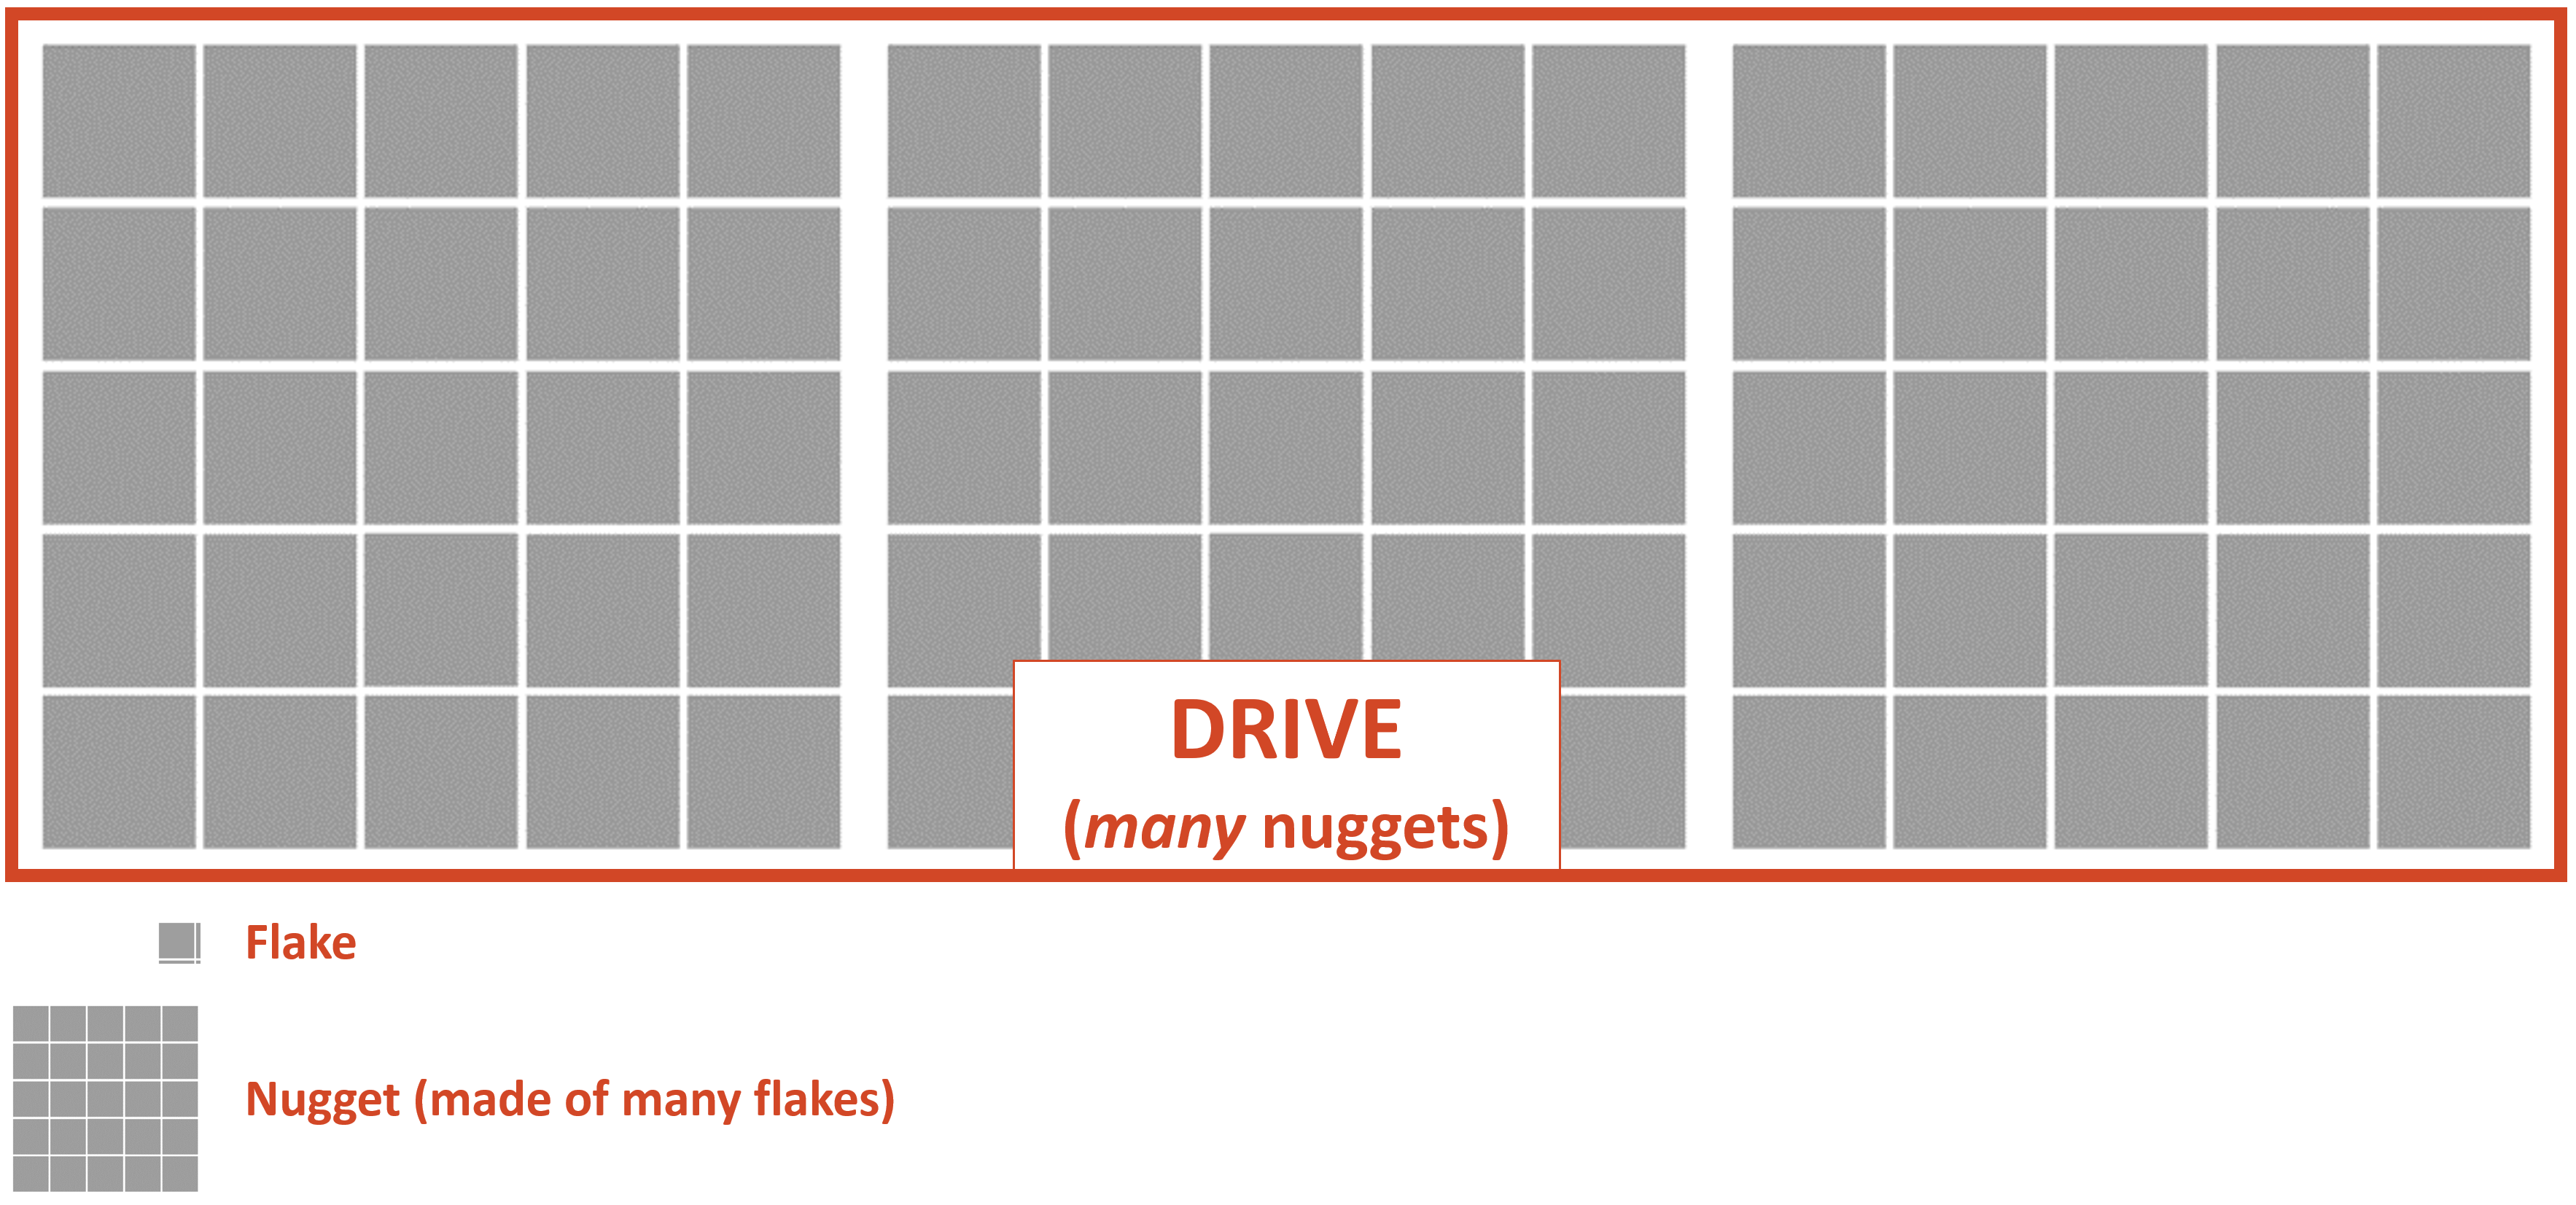
\includegraphics[width=\linewidth]{flknug.png}
   \caption{Anatomy of a StrongBox nugget.}\label{fig:flknug}
\end{figure}

StrongBox divides the underlying drive into a series same-size logical blocks
called \emph{nuggets}, illustrated in \figref{flknug}. A nugget consists of one
or more physical drive blocks/sectors, depending on its configured size. Each
nugget is subdivided into a constant number of units called \emph{flakes}.

StrongBox uses this flake-nugget structure to 1) track, detect, and handle
overwrites and 2) limit the maximum length of any plaintexts provided to
ciphers, thus capping the overhead incurred during expensive re-keying
operations when overwrites do occur.

\subsection{Key Insights}

\subsubsection{A Single Point In A Space Of Possible Cipher Configurations}
\TODO{This is an example of why we need to make sure that our claims are stronger than just making strongbox better.  It would be great to ask what if the above schemes used a range of ciphers?  And then make the text of this paragraph more general for all types of stream-cipher based fde.}
What if we used StrongBox with ciphers \textit{other} than ChaCha20? Redesigning
StrongBox with a generic cipher API allows for ciphers other than ChaCha20 to be
used, yielding a space of cipher configuration points with various performance,
battery life, security, drive space, and other tradeoffs. It follows then that
the original StrongBox construction using ChaCha20 exists as one point in this
space of cipher configurations.

\begin{figure}[ht] \textbf{Baseline Cipher I/O Performance}\par\medskip
   \centering
   {\begin{tikzpicture}[baseline]

    \pgfmathsetmacro{\ymax}{1.1} % set the maximum y value
    \pgfmathsetmacro{\ymaxbreak}{1.2} % set the y value at which overflow is drawn

    \begin{groupplot}[
        group style={
            group size=2 by 2,
            xlabels at=edge bottom,
            ylabels at=edge left,
            xticklabels at=edge bottom,
            yticklabels at=edge left,
            vertical sep=25pt,
            horizontal sep=15pt,
        },
        %axis x line*=bottom,
        height=3.5cm,
        width=\linewidth/1.5,
        tick align=outside,
        tick pos=bottom, % make sure ticks only appear at the bottom and left axes
        title style={yshift=-1.5ex},
        tick style={ black },
        y tick label style={ /pgf/number format/fixed, /pgf/number format/precision=0 },
        grid style={ dotted, gray },
        scatter,
        point meta=explicit symbolic,
        scatter/classes={
            c8={mark=square*},
            c20={mark=triangle*},
            ff={mark=diamond*},
            fb={mark=pentagon*},
            fs={mark=otimes}
        },
        %every node near coord/.append style={font=\tiny},
        %
        % magic to make the numbers appear above the overly long bars:
        % visualization depends on={rawy \as \rawy}, % save original y values
        % restrict y to domain*={ % now clip/restrict any y value to ymax
        %     \pgfkeysvalueof{/pgfplots/ymin}:\ymaxbreak
        % },
        % after end axis/.code={ % draw squiggly line indicating break
        %     \draw [semithick, white, decoration={snake,amplitude=0.1mm,segment length=0.75mm,post length=0.375mm}, decorate] (rel axis cs:0,1.01) -- (rel axis cs:1,1.01);
        % },
        % nodes near coords={\color{.!75!black}\pgfmathprintnumber\rawy}, % print the original y values (darkened in case they are too light)...
        % nodes near coords greater equal only=\ymax, % ... but ONLY if they are >= ymax
        % clip=false, % allow clip to protrude beyond ymax
        % Custom stuff to edit per template
        %
        xlabel={\footnotesize Security Score},
        xlabel near ticks,
        %xlabel shift={-1.5mm},
        xmin=0, xmax=4,
        xtick={ 0, 1, 2, 3, 4 },
        xticklabels={ 0,,, 3, \empty },
        %major x tick style=transparent,
        %enlarge x limits=0.2, % add some breathing room along the x axis's sides
        %
        ylabel={\footnotesize Latency (normalized)},
        ylabel near ticks,
        ylabel shift={-1.5mm},
        ymajorgrids=true,
        ymin=0, ymax=\ymax,
        ytick={ 0, 1, \ymax },
        yticklabels={ 0, 1, \empty },
        %yticklabels={ 0, 0.5, 1.5, 2 },
        % extra y ticks={1},
        % extra y tick style={grid=major, grid style={dashed, black}},
        % extra y tick label={\empty},
        %bar width=4.5pt, % change size of bars
        %
        legend cell align=center,
        legend style={ column sep=1ex },
        legend entries={%
            {\scriptsize 4K},
            {\scriptsize 512K},
            {\scriptsize 5M},
            {\scriptsize 40M}
        },
        legend style={
            draw=none,
            legend columns=4,
            at={(1.0,1.35)},
            anchor=south,
        },
    ]
        \nextgroupplot[title={Sequential Reads}]
            \addlegendimage{no markers,red}
            \addlegendimage{no markers,green,dashed}
            \addlegendimage{no markers,blue,dashdotted}
            \addlegendimage{no markers,orange,densely dotted}
            \addplot [thick, red] table [
                meta=cipher,
                x=score,
                y=latency,
                discard if symbol not={iop}{4k-r},
                discard if symbol not={order}{seq},
                col sep=space,
            ] {charts/tradeoff-baseline.dat};
            % \label[c8]{fig:tnr:c8}
            % \label[c20]{fig:tnr:c20}
            % \label[ff]{fig:tnr:ff}
            % \label[fb]{fig:tnr:fb}
            % \label[fs]{fig:tnr:fs}
            \addplot [thick, dashed, green] table [
                meta=cipher,
                x=score,
                y=latency,
                discard if symbol not={iop}{512k-r},
                discard if symbol not={order}{seq},
                col sep=space
            ] {charts/tradeoff-baseline.dat};
            \addplot [thick, dashdotted, blue] table [
                meta=cipher,
                x=score,
                y=latency,
                discard if symbol not={iop}{5m-r},
                discard if symbol not={order}{seq},
                col sep=space
            ] {charts/tradeoff-baseline.dat};
            \addplot [thick, densely dotted, orange] table [
                meta=cipher,
                x=score,
                y=latency,
                discard if symbol not={iop}{40m-r},
                discard if symbol not={order}{seq},
                col sep=space
            ] {charts/tradeoff-baseline.dat};
        \nextgroupplot[legend to name={throwaway1}, title={Random Reads}]
            \addplot [thick, red] table [
                meta=cipher,
                x=score,
                y=latency,
                discard if symbol not={iop}{4k-r},
                discard if symbol not={order}{rnd},
                col sep=space,
            ] {charts/tradeoff-baseline.dat};
            \addplot [thick, dashed, green] table [
                meta=cipher,
                x=score,
                y=latency,
                discard if symbol not={iop}{512k-r},
                discard if symbol not={order}{rnd},
                col sep=space
            ] {charts/tradeoff-baseline.dat};
            \addplot [thick, dashdotted, blue] table [
                meta=cipher,
                x=score,
                y=latency,
                discard if symbol not={iop}{5m-r},
                discard if symbol not={order}{rnd},
                col sep=space
            ] {charts/tradeoff-baseline.dat};
            \addplot [thick, densely dotted, orange] table [
                meta=cipher,
                x=score,
                y=latency,
                discard if symbol not={iop}{40m-r},
                discard if symbol not={order}{rnd},
                col sep=space
            ] {charts/tradeoff-baseline.dat};
        \nextgroupplot[legend to name={throwaway2}, title={Sequential Writes}]
            \addplot [thick, red] table [
                meta=cipher,
                x=score,
                y=latency,
                discard if symbol not={iop}{4k-w},
                discard if symbol not={order}{seq},
                col sep=space,
            ] {charts/tradeoff-baseline.dat};
            \addplot [thick, dashed, green] table [
                meta=cipher,
                x=score,
                y=latency,
                discard if symbol not={iop}{512k-w},
                discard if symbol not={order}{seq},
                col sep=space
            ] {charts/tradeoff-baseline.dat};
            \addplot [thick, dashdotted, blue] table [
                meta=cipher,
                x=score,
                y=latency,
                discard if symbol not={iop}{5m-w},
                discard if symbol not={order}{seq},
                col sep=space
            ] {charts/tradeoff-baseline.dat};
            \addplot [thick, densely dotted, orange] table [
                meta=cipher,
                x=score,
                y=latency,
                discard if symbol not={iop}{40m-w},
                discard if symbol not={order}{seq},
                col sep=space
            ] {charts/tradeoff-baseline.dat};
        \nextgroupplot[legend to name={throwaway3}, title={Random Writes}]
            \addplot [thick, red] table [
                meta=cipher,
                x=score,
                y=latency,
                discard if symbol not={iop}{4k-w},
                discard if symbol not={order}{rnd},
                col sep=space,
            ] {charts/tradeoff-baseline.dat};
            \addplot [thick, dashed, green] table [
                meta=cipher,
                x=score,
                y=latency,
                discard if symbol not={iop}{512k-w},
                discard if symbol not={order}{rnd},
                col sep=space
            ] {charts/tradeoff-baseline.dat};
            \addplot [thick, dashdotted, blue] table [
                meta=cipher,
                x=score,
                y=latency,
                discard if symbol not={iop}{5m-w},
                discard if symbol not={order}{rnd},
                col sep=space
            ] {charts/tradeoff-baseline.dat};
            \addplot [thick, densely dotted, orange] table [
                meta=cipher,
                x=score,
                y=latency,
                discard if symbol not={iop}{40m-w},
                discard if symbol not={order}{rnd},
                col sep=space
            ] {charts/tradeoff-baseline.dat};
    \end{groupplot}%
\end{tikzpicture}%
} \caption{Median sequential and random
   read and write latency per I/O operation size (4KB, 512KB, 5MB, 40MB) using
   multiple cipher configurations achievable without switching and ordered by
   security score.}
  \label{fig:tradeoff-no-ratios}
\end{figure}

\TODO{You have to introduce the scoring before you get here.  Or at least introduce the notion of scoring with citations. or that the community agrees on the relative strength with citations.}
For instance, \figref{tradeoff-no-ratios} shows the security versus I/O latency
tradeoff between different stream ciphers (including ChaCha20) when completing a
40MB read of encrypted storage. The experiment was performed on a Linux RAM disk
on an ARM big.LITTLE Exynos Octa processor, which is similar to the processors
used in the Samsung Galaxy line of phones and other devices. Of the ciphers we
tested, those with more desirable but performance inhibitive security guarantees
(see: \secref{design}) resulted in higher latency for I/O operations while
ciphers with relatively weaker less desirable security guarantees resulted in
lower latency.

\subsubsection{Nugget Encryption/Decryption And Re-Keying Is Entirely Independent}

With SwitchBox, nuggets are considered as distinct logical blocks, each with
their own metadata and unique cryptographic key used to encrypt and decrypt
their contents independent of other nuggets using the cipher chosen at system
initialization. This layout of distinct logical blocks naturally lends itself to
encrypting different portions of the underlying drive with different ciphers
instead; we can select any cipher to encrypt or decrypt any nugget at any point,
rather than just a single cipher applied globally across the backing store. This
design supports mixed cipher configurations such that each nugget can be encrypted,
decrypted, and switched independently from all other nuggets.

\subsubsection{Navigate The Configuration Space With \emph{Cipher Switching}}

Given a space of possible cipher configurations and a drive layout of
independent nuggets that lends itself to mixed cipher use, it is clear our
system does not have to sit at a static configuration point. Hence, we require a
mechanism to navigate the cipher configuration space, trading off concerns such
that the system is always at the most optimal configuration given the runtime
environment and user requirements. By abstracting the re-keying process out into a \emph{re-ciphering}
or \emph{cipher switching} process, whereby the key and the cipher used to
encrypt/decrypt the nugget can both be switched at runtime, we can trade off
between different ciphers and their characteristics dynamically. Comparatively,
prior work can only accomplish a static tradeoff at compile time or at system
initialization. \\
\\
Leveraging these insights, we present SwitchBox. \TODO{A few short explanatory
sentences that lead to: Our goal is to dynamically trade desirable security
properties for performance or energy.}

\subsection{Motivating Example: Filesystem Reacts to OS ``Power Saver'' Mode}

\begin{figure}[ht] \textbf{Linearity Between Baseline Cipher Latency and Energy
Use}\par\medskip
   \centering
   {\begin{tikzpicture}[baseline]

    \pgfmathsetmacro{\ymax}{1} % set the maximum y value
    \pgfmathsetmacro{\ymaxbreak}{1.1} % set the y value at which overflow is drawn

    \begin{axis}[
        %axis x line*=bottom,
        only marks,
        height=6cm,
        width=\linewidth,
        tick align=outside,
        tick pos=bottom, % make sure ticks only appear at the bottom and left axes
        tick style={ black },
        y tick label style={ /pgf/number format/fixed, /pgf/number format/precision=0 },
        grid style={ dotted, gray },
        %every node near coord/.append style={font=\tiny},
        %
        % magic to make the numbers appear above the overly long bars:
        % visualization depends on={rawy \as \rawy}, % save original y values
        % restrict y to domain*={ % now clip/restrict any y value to ymax
        %     \pgfkeysvalueof{/pgfplots/ymin}:\ymaxbreak
        % },
        % after end axis/.code={ % draw squiggly line indicating break
        %     \draw [semithick, white, decoration={snake,amplitude=0.1mm,segment length=0.75mm,post length=0.375mm}, decorate] (rel axis cs:0,1.01) -- (rel axis cs:1,1.01);
        % },
        % nodes near coords={\color{.!75!black}\pgfmathprintnumber\rawy}, % print the original y values (darkened in case they are too light)...
        % nodes near coords greater equal only=\ymax, % ... but ONLY if they are >= ymax
        % clip=false, % allow clip to protrude beyond ymax
        % Custom stuff to edit per template
        %
        xlabel={\footnotesize Energy (normalized)},
        xlabel near ticks,
        xmin=0, xmax=1,
        xtick={ 0, 1 },
        %enlarge x limits=0.2, % add some breathing room along the x axis's sides
        %major x tick style=transparent,
        %
        ylabel={\footnotesize Latency (normalized)},
        ylabel near ticks,
        ylabel shift={-1mm},
        ymajorgrids=true,
        ymin=0, ymax=\ymax,
        ytick={ 0, 1 },
        restrict x to domain=0:1,
        %yticklabels={ 0, 0.5, 1.5, 2 },
        % extra y ticks={1},
        % extra y tick style={grid=major, grid style={dashed, black}},
        % extra y tick label={\empty},
        %bar width=4.5pt, % change size of bars
        %
        legend cell align=left,
        legend style={ column sep=1ex },
        legend style={
            draw=none,
            legend columns=2,
            at={(0.5,1.02)},
            anchor=south,
        },
    ]
        \addplot [blue] table [
            only marks,
            x=energy,
            y=latency,
            discard if symbol not={iop}{4k-r},
            discard if symbol not={order}{seq},
            col sep=space,
        ] {charts/tradeoff-baseline.dat};
        \addlegendentry{\scriptsize 4K I/O}
        \addplot [] table [
            only marks,
            x=energy,
            y=latency,
            discard if symbol not={iop}{512k-r},
            discard if symbol not={order}{seq},
            col sep=space
            ] {charts/tradeoff-baseline.dat};
        \addlegendentry{\scriptsize 512K/5M/40M I/O}
        \addlegendimage{mark=none, red, thick}
        \addlegendentry{\scriptsize Regression}
        \addplot [] table [
            only marks,
            x=energy,
            y=latency,
            discard if symbol not={iop}{5m-r},
            discard if symbol not={order}{seq},
            col sep=space
        ] {charts/tradeoff-baseline.dat};
        \addplot [] table [
            only marks,
            x=energy,
            y=latency,
            discard if symbol not={iop}{40m-r},
            discard if symbol not={order}{seq},
            col sep=space
        ] {charts/tradeoff-baseline.dat};
        \addplot [blue] table [
            only marks,
            x=energy,
            y=latency,
            discard if symbol not={iop}{4k-w},
            discard if symbol not={order}{rnd},
            col sep=space,
        ] {charts/tradeoff-baseline.dat};
        \addplot [] table [
            only marks,
            x=energy,
            y=latency,
            discard if symbol not={iop}{512k-w},
            discard if symbol not={order}{rnd},
            col sep=space
        ] {charts/tradeoff-baseline.dat};
        \addplot [] table [
            only marks,
            x=energy,
            y=latency,
            discard if symbol not={iop}{5m-w},
            discard if symbol not={order}{rnd},
            col sep=space
        ] {charts/tradeoff-baseline.dat};
        \addplot [] table [
            only marks,
            x=energy,
            y=latency,
            discard if symbol not={iop}{40m-w},
            discard if symbol not={order}{rnd},
            col sep=space
        ] {charts/tradeoff-baseline.dat};
        \addplot [sharp plot, mark=none, red] table [
            x=energy,
            y={create col/linear regression={y=latency}},
            col sep=space
        ] {charts/tradeoff-baseline.dat};
    \end{axis}%
\end{tikzpicture}%
} \caption{Comparison of cipher
   configuration median sequential and random latency versus median total energy
   use per I/O operation size (4KB, 512KB, 5MB, 40MB) without switching. The
   relationship between latency and total energy use is linear for the cipher
   configurations we examine in this paper.}
  \label{fig:linearity-latency-energy}
\end{figure}

Suppose we are continually streaming a high-resolution video stored on our
mobile device to several WiFi connected devices, such as televisions or
projectors. We stored the video and other data on our device drive as securely
as possible, so we chose to initialize the system at a configuration point
offering very strong security.

For the ciphers examined in this paper, \figref{linearity-latency-energy} shows
a correlation between stronger security guarantees and greater total energy use,
meaning our device is using a lot more energy to facilitate FDE at this
configuration point. Though this correlation applies to the ciphers we examined,
note that this correlation is certainly not true for all possible ciphers.

Further suppose that, after a while of streaming, our device determines its
remaining battery life is too low and enters a ``power saver'' mode with a
curtailed energy budget. With a traditional filesystem or encrypted container,
we are stuck with our high-energy configuration chosen at system initialization.

However, with the ability to operate at points along the pareto frontier (see
\figref{tradeoff-no-ratios}), even at points between the discrete configurations
available to prior work, a context-aware system can switch to a configuration
that trades the security of the portions of storage that are being used to
stream the video so that we stay within our curtailed energy budget.

When we return to a non-curtailed energy budget, the system can return to its
more secure configuration dynamically, allowing the cipher strength of the
backing store to eventually recover without having to recreate the entire
underlying filesystem or encrypted container.

\TODO{How does this example work?  If the video is originally stored with high security, then don't we have to decrypt it first and then re-encrypt at a different level?  Isn't the cost the read from high-security state?  I think we talked about this a while ago, but I don't remember the details.  My forgetfulness is actually good, because I can tell you that this example isn't going to do it without a lot more detail about why switching actually helps here.}

\subsection{Challenges}

\textbf{Comparing ciphers with disparate security guarantees.} To ensure that
these tradeoffs are made optimally, it is desirable to score the security
properties of various ciphers. This is challenging since different ciphers have
a wide range of energy/latency vs security properties, including ciphers that
are and are not length-preserving. Hence, cipher configurations will not form a
continuous tradeoff space in any scheme and so represent discrete points, yet
the desired energy, latency, or security state may lie between these points.

To address this, we propose a method for quantitative cipher comparison in the
FDE context, and then present some empirical results showing the wide range of
security and energy tradeoffs that become available with various
state-of-the-art ciphers as a result.\\
\\
\textbf{Maintaining I/O performance with a mixed-cipher drive layout.} With
prior work, cipher configurations are typically fixed at the time the system is
booted or the filesystem or container is created~\cite{CiteAllTheFilesystems};
if requirements change online, at best the entire system requires a reboot leading to down time and user dissatisfaction. 
At worst, before the reboot, the filesystem or encrypted
container has to be deleted and recreated. This is rarely desirable. Hence,
SwitchBox requires a generic \emph{cipher API}, IPC, and a software mechanism
that can re-cipher or \emph{switch} the cipher used to encrypt and decrypt
individual nuggets while maintaining low overhead and acceptable performance.
This mechanism should allow for a mixed-cipher drive layout and provides the
``how'' to switch nuggets' ciphers.

To provide the ``when'' or ``where'', we implement and demonstrate a series of
novel cipher switching \textit{strategies} that, along with the ``pluggable''
cipher API and cipher switching mechanism, enable optimal navigation of the
tradeoff space of configurations. For instance, these strategies allow SwitchBox
to settle on points between the static cipher configurations in
\figref{tradeoff-no-ratios}.

\TODO{Might be able to piece this out into two challenges: common interface for
stream ciphers and cipher switching strategies; that last one might be able to
split into two on its own. Perhaps this challenge subsection should mirror the
layout of the design section?}
